\documentclass[a4paper,twoside]{article}
\usepackage{blindtext}  
\usepackage{geometry}

% Chinese support
\usepackage[UTF8, scheme = plain]{ctex}

% Page margin layout
\geometry{left=2.3cm,right=2cm,top=2.5cm,bottom=2.0cm}


\usepackage{listings}
\usepackage{xcolor}
\usepackage{geometry}
\usepackage{amsmath}
\usepackage{float}
\usepackage{hyperref}

\usepackage{graphics}
\usepackage{graphicx}
\usepackage{subcaption}
\usepackage{epsfig}
\usepackage{float}

\usepackage{algorithm}
\usepackage[noend]{algpseudocode}

\usepackage{booktabs}
\usepackage{threeparttable}
\usepackage{longtable}
\usepackage{tikz}
\usepackage{multicol}
\usepackage{pgfplots}
\pgfplotsset{compat=1.9}
\pgfplotsset{
    myplotstyle/.style={
    legend style={draw=none, font=\small},
    legend cell align=left,
    legend pos=north east,
    ylabel style={align=center, font=\bfseries\boldmath},
    xlabel style={align=center, font=\bfseries\boldmath},
    x tick label style={font=\bfseries\boldmath},
    y tick label style={font=\bfseries\boldmath},
    scaled ticks=false,
    every axis plot/.append style={thick},
    },
}

% cite package, to clean up citations in the main text. Do not remove.
\usepackage{cite}

\usepackage{color,xcolor}

%% The amssymb package provides various useful mathematical symbols
\usepackage{amssymb}
%% The amsthm package provides extended theorem environments
\usepackage{amsthm}
\usepackage{amsfonts}
\usepackage{enumerate}
\usepackage{enumitem}
\usepackage{listings}
\usepackage{minted}


\usepackage{indentfirst}
\setlength{\parindent}{2em} % Make two letter space in the first paragraph
\usepackage{setspace}
\linespread{1.5} % Line spacing setting
\usepackage{siunitx}
\setlength{\parskip}{0.5em} % Paragraph spacing setting

% \usepackage[contents =22920202204622, scale = 10, color = black, angle = 50, opacity = .10]{background}

\renewcommand{\figurename}{图}
\renewcommand{\listingscaption}{代码}
\renewcommand{\tablename}{表格}
\renewcommand{\contentsname}{目录}
\floatname{algorithm}{算法}

\graphicspath{ {images/} }

%%%%%%%%%%%%%
\newcommand{\StudentNumber}{22920202204622}  % Fill your student number here
\newcommand{\StudentName}{熊恪峥}  % Replace your name here
\newcommand{\PaperTitle}{实验(四)内存管理}  % Change your paper title here
\newcommand{\PaperType}{操作系统实验报告} % Replace the type of your report here
\newcommand{\Date}{2023年6月5日}
\newcommand{\College}{信息学院}
\newcommand{\CourseName}{操作系统}
%%%%%%%%%%%%%

%% Page header and footer setting
\usepackage{fancyhdr}
\usepackage{lastpage}
\pagestyle{fancy}
\fancyhf{}
% This requires the document to be twoside
\fancyhead[LO]{\texttt{\StudentName }}
\fancyhead[LE]{\texttt{\StudentNumber}}
\fancyhead[C]{\texttt{\PaperTitle }}
\fancyhead[R]{\texttt{第{\thepage}页,共\pageref*{LastPage}页}}


\title{\PaperTitle}
\author{\StudentName}
\date{\Date}

\algnewcommand\algorithmicinput{\textbf{Input:}}
\algnewcommand\algorithmicoutput{\textbf{Output:}}
\algnewcommand\Input{\item[\algorithmicinput]}%
\algnewcommand\Output{\item[\algorithmicoutput]}%

\usetikzlibrary{positioning, shapes.geometric,arrows,automata}

\tikzstyle{startstop} = [rectangle, rounded corners, minimum width=3cm, minimum height=1cm, text centered, draw=black, fill=red!30]
\tikzstyle{io} = [trapezium, trapezium left angle=70, trapezium right angle=110, minimum width=3cm, minimum height=1cm, text centered, draw=black, fill=blue!30]
\tikzstyle{process} = [rectangle, minimum width=3cm, minimum height=1cm, text centered, draw=black, fill=green!30]
\tikzstyle{decision} = [diamond, minimum width=3cm, minimum height=1cm, text centered, draw=black, fill=yellow!30]
\tikzstyle{arrow} = [thick,->,>=stealth]

\begin{document}
	
%%%%%%%%%%%%%%%%%%%%%%%%%%%%%%%%%%%%%%%%%%%%
\makeatletter % change default title style
\renewcommand*\maketitle{%
	\begin{center} 
		\bfseries  % title 
		{\LARGE \@title \par}  % LARGE typesetting
		\vskip 1em  %  margin 1em
		{\global\let\author\@empty}  % no author information
		{\global\let\date\@empty}  % no date
		\thispagestyle{empty}   %  empty page style
	\end{center}%
	\setcounter{footnote}{0}%
}
\makeatother
%%%%%%%%%%%%%%%%%%%%%%%%%%%%%%%%%%%%%%%%%%%%
	
	
\thispagestyle{empty}

\vspace*{1cm}

\begin{figure}[htb]
	\centering
	
\includegraphics[width=4.0cm]{logo.png}
\end{figure}

\vspace*{1cm}

\begin{center}
	\Huge{\textbf{\PaperType}}
	
	\Large{\PaperTitle}
\end{center}

\vspace*{1cm}

\begin{table}[H]
	\centering	
	\begin{Large}
		\renewcommand{\arraystretch}{1.5}
		\begin{tabular}{p{3cm} p{5cm}<{\centering}}
			姓\qquad 名 & \StudentName  \\
			\hline
			学\qquad号 & \StudentNumber \\
			\hline
			日\qquad期 & \Date  \\
			\hline
			学\qquad院 & \College  \\
			\hline
			课程名称 & \CourseName  \\
			\hline
		\end{tabular}
	\end{Large}
\end{table}

\newpage

\title{
	\Large{\textcolor{black}{\PaperTitle}}
}

\maketitle
	
\tableofcontents
 
\newpage
\setcounter{page}{1}

\begin{spacing}{1.2}

\section{实验内容}

本实验利用内核函数 \texttt{kmalloc()},\texttt{ vmalloc()}实现内存的分配,并要求学生根据提示实现基于最佳适应算法的\texttt{bf\_malloc}内存分配器。  

\section{实验目的}

\begin{enumerate}
	\item 学习掌握\texttt{kmalloc()}和\texttt{vmalloc()}分配内存的差异;
	\item 加深对首次适应算法和最佳适应算法的理解;
	\item 锻炼编写内核模块的能力。
\end{enumerate}

\section{使用\texttt{kmalloc}分配内存}

\texttt{kmalloc}具有两个参数,第一个参数是要分配的内存大小,第二个参数是分配内存的类型。
在本次实验中,我们使用\texttt{GFP\_KERNEL}来在内核空间分配内存。
该函数失败时会返回\texttt{NULL},因此我们需要检查返回值是否为\texttt{NULL},如果是则说明分配失败,
则输出错误信息“Failed to allocate kmallocmem1/ kmallocmem2/ kmallocmem3 / kmallocmem4!”。

根据以上思路,编写代码~\ref{code:kmalloc}。
\begin{listing}[htb]
	\caption{使用\texttt{kmalloc}分配内存}
	\label{code:kmalloc}
	\inputminted[firstline=14,lastline=42]{c}{../code/1/1.c}
\end{listing}
代码~\ref{code:kmalloc}将在模块加载时执行,遇到错误输出错误消息,否则输出分配内存的大小。
代码的运行结果如图~\ref{fig:kmalloc}所示。
\begin{figure}[htb]
	\centering
	\caption{使用\texttt{kmalloc}分配内存}
	\label{fig:kmalloc}
	\begin{subfigure}{0.45\textwidth}
		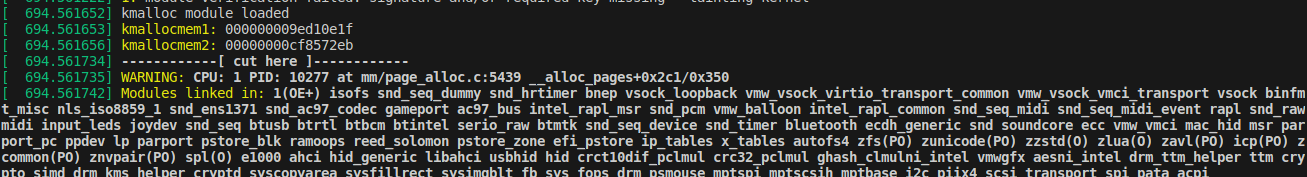
\includegraphics[width=0.9\textwidth]{images/km1.png}
	\end{subfigure}
	\begin{subfigure}{0.45\textwidth}
		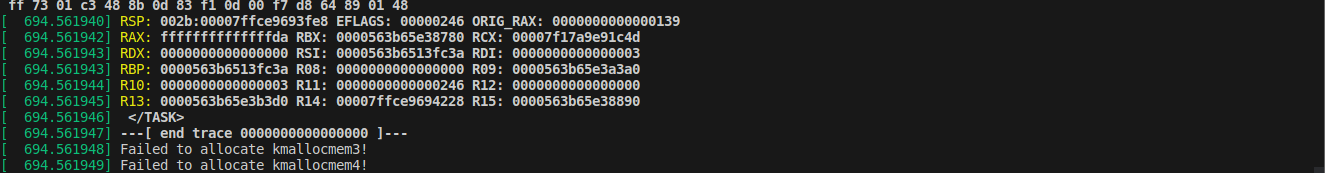
\includegraphics[width=0.9\textwidth]{images/km2.png}
	\end{subfigure}
\end{figure}

可见,前两个请求成功了,而后两个请求失败了。

\subsection{\texttt{kmalloc}的分配上限}

常识告诉我们,由于kmalloc分配时需要保证有连续的物理内存页一定空闲,所以一定具有上限。
同时,查阅Linux内核文档,可以发现如下内容:
\begin{quotation}
	The maximal size of a chunk that can be allocated with kmalloc is limited. The actual limit depends on the hardware and the kernel configuration, but it is a good practice to use kmalloc for objects smaller than page size.
\end{quotation}
因此,确实具有上限。

首先,为了找到上限,可以修改代码~\ref{code:kmalloc}。
通过不断修改\texttt{kmallocmem3}和\texttt{kmallocmem4}的大小,
保证前者请求成功,后者请求失败,并逐步减半区间长度,可以快速逼近得到上限。
根据以上过程,得到了上限是4MB。

同时,该值也可以从内核源码中得到依据:查看\texttt{include/linux/slab.h}文件,其中定义
宏\texttt{KMALLOC\_MAX\_SIZE}为\texttt{(1UL << KMALLOC\_SHIFT\_HIGH)},而宏
\texttt{KMALLOC\_SHIFT\_HIGH}又定义为:
\begin{minted}{c}
#define KMALLOC_SHIFT_HIGH      ((MAX_ORDER + PAGE_SHIFT - 1) <= 25 ? \
                               (MAX_ORDER + PAGE_SHIFT - 1) : 25)
\end{minted}
在x86架构下,\texttt{MAX\_ORDER}为11,\texttt{PAGE\_SHIFT}为12,因此可以计算得出:
\begin{equation}
	\texttt{KMALLOC\_MAX\_SIZE} = 2^{11+12-1} = 4\texttt{MB}
\end{equation}
同时,这也说明了在任何架构下,\texttt{KMALLOC\_MAX\_SIZE}都不能超过32MB。因为宏\texttt{KMALLOC\_SHIFT\_HIGH}
保证了该值不超过$2^{25}\texttt{B}=32\texttt{MB}$。

\subsection{分配区域}

由于指定了分配内存的类型为\texttt{GFP\_KERNEL},因此分配的内存位于内核空间,分配的物理地址会处于896MB之下(32位架构),
然后根据Linux内核的内存管理机制,会将这些物理地址映射到2GB之上。这符合图~\ref{fig:mem}中的结果。

\section{使用\texttt{vmalloc}分配内存}

\texttt{vmalloc}可以分配虚拟连续的内存,但是不能保证物理连续。
这降低了对物理内存的要求。编写代码非常简单,只需将代码~\ref{code:kmalloc}中的\texttt{kmalloc}替换为\texttt{vmalloc}即可。
例如分配\texttt{vmallocmem1}时,代码如下:
\begin{listing}[htb]
	\caption{使用\texttt{kmalloc}分配内存}
	\label{code:kmalloc}
	\inputminted[firstline=17,lastline=22]{c}{../code/2/2.c}
\end{listing}

运行结果如图~\ref{fig:vmalloc}所示。
\begin{figure}[htb]
	\centering
	\caption{使用\texttt{vmalloc}分配内存}
	\label{fig:vmalloc}
	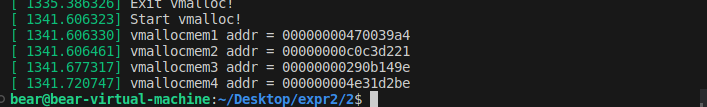
\includegraphics[width=0.9\textwidth]{images/vm.png}
\end{figure}
可见,\texttt{vmalloc}可以成功分配远大于上述\texttt{kmalloc}上限的内存。
因为真正对物理内存页的分配被推迟到了第一次访问时。这既增加了分配的灵活性,也会带来无法用于DMA等问题。

\subsection{分配区域}

\texttt{vmalloc}可以分配虚拟连续的内存,但是不能保证物理连续。而\texttt{kmalloc}则要求物理连续的页面。
\texttt{vmalloc}会将内存地址分配到单独的一个区域,这个区域由宏\texttt{VMALLOC\_START}和\texttt{VMALLOC\_END}指定。
在i386架构(32位)下会优先选择\texttt{ZONE\_HIGHMEM},否则会选择\texttt{ZONE\_NORMAL},在图~\ref{fig:vmalloc}中,
由于默认使用了32位编译,所以符合这种情况,分配的地址在\texttt{0xc0000000}附近。

在64位x86架构下,由于地址空间大大扩展了,因此分配的区域也更大,该区域处在地址的Canonical Bits为1的区域,处在内存空间较高的位置,
根据文档\footnote{\url{https://elixir.bootlin.com/linux/v5.0/source/Documentation/x86/x86_64/mm.txt}},
该区域的起始地址为\texttt{ffffc90000000000},结束地址为\texttt{ffffe8ffffffffff}。

\section{阅读并理解首次适应算法的实现}

首先,内存分配器使用结构\texttt{header}进行管理:
\inputminted[firstline=10,lastline=18]{c}{../code/3/ff_malloc.c}
它记录了每一个空闲块的长度和下一块的位置。能够把内存块通过链表的方式进行记录和管理。
具体的链表头为\texttt{list}指针。

\subsection{\texttt{ff\_malloc}}

\texttt{ff\_malloc}为内存分配的具体逻辑,用于分配\texttt{size}大小的内存。
同时,如果未初始化,也会初始化链表和相应的指针。
初始化完成后,就会查找第一个适配的块并进行拆分,如果没有这样的块就再调用\texttt{sbrk}进行分配。
具体流程如图~\ref{fig:ff}。

\begin{figure}[htb]
	\centering
	\caption{首次适配算法}
	\label{fig:ff}
	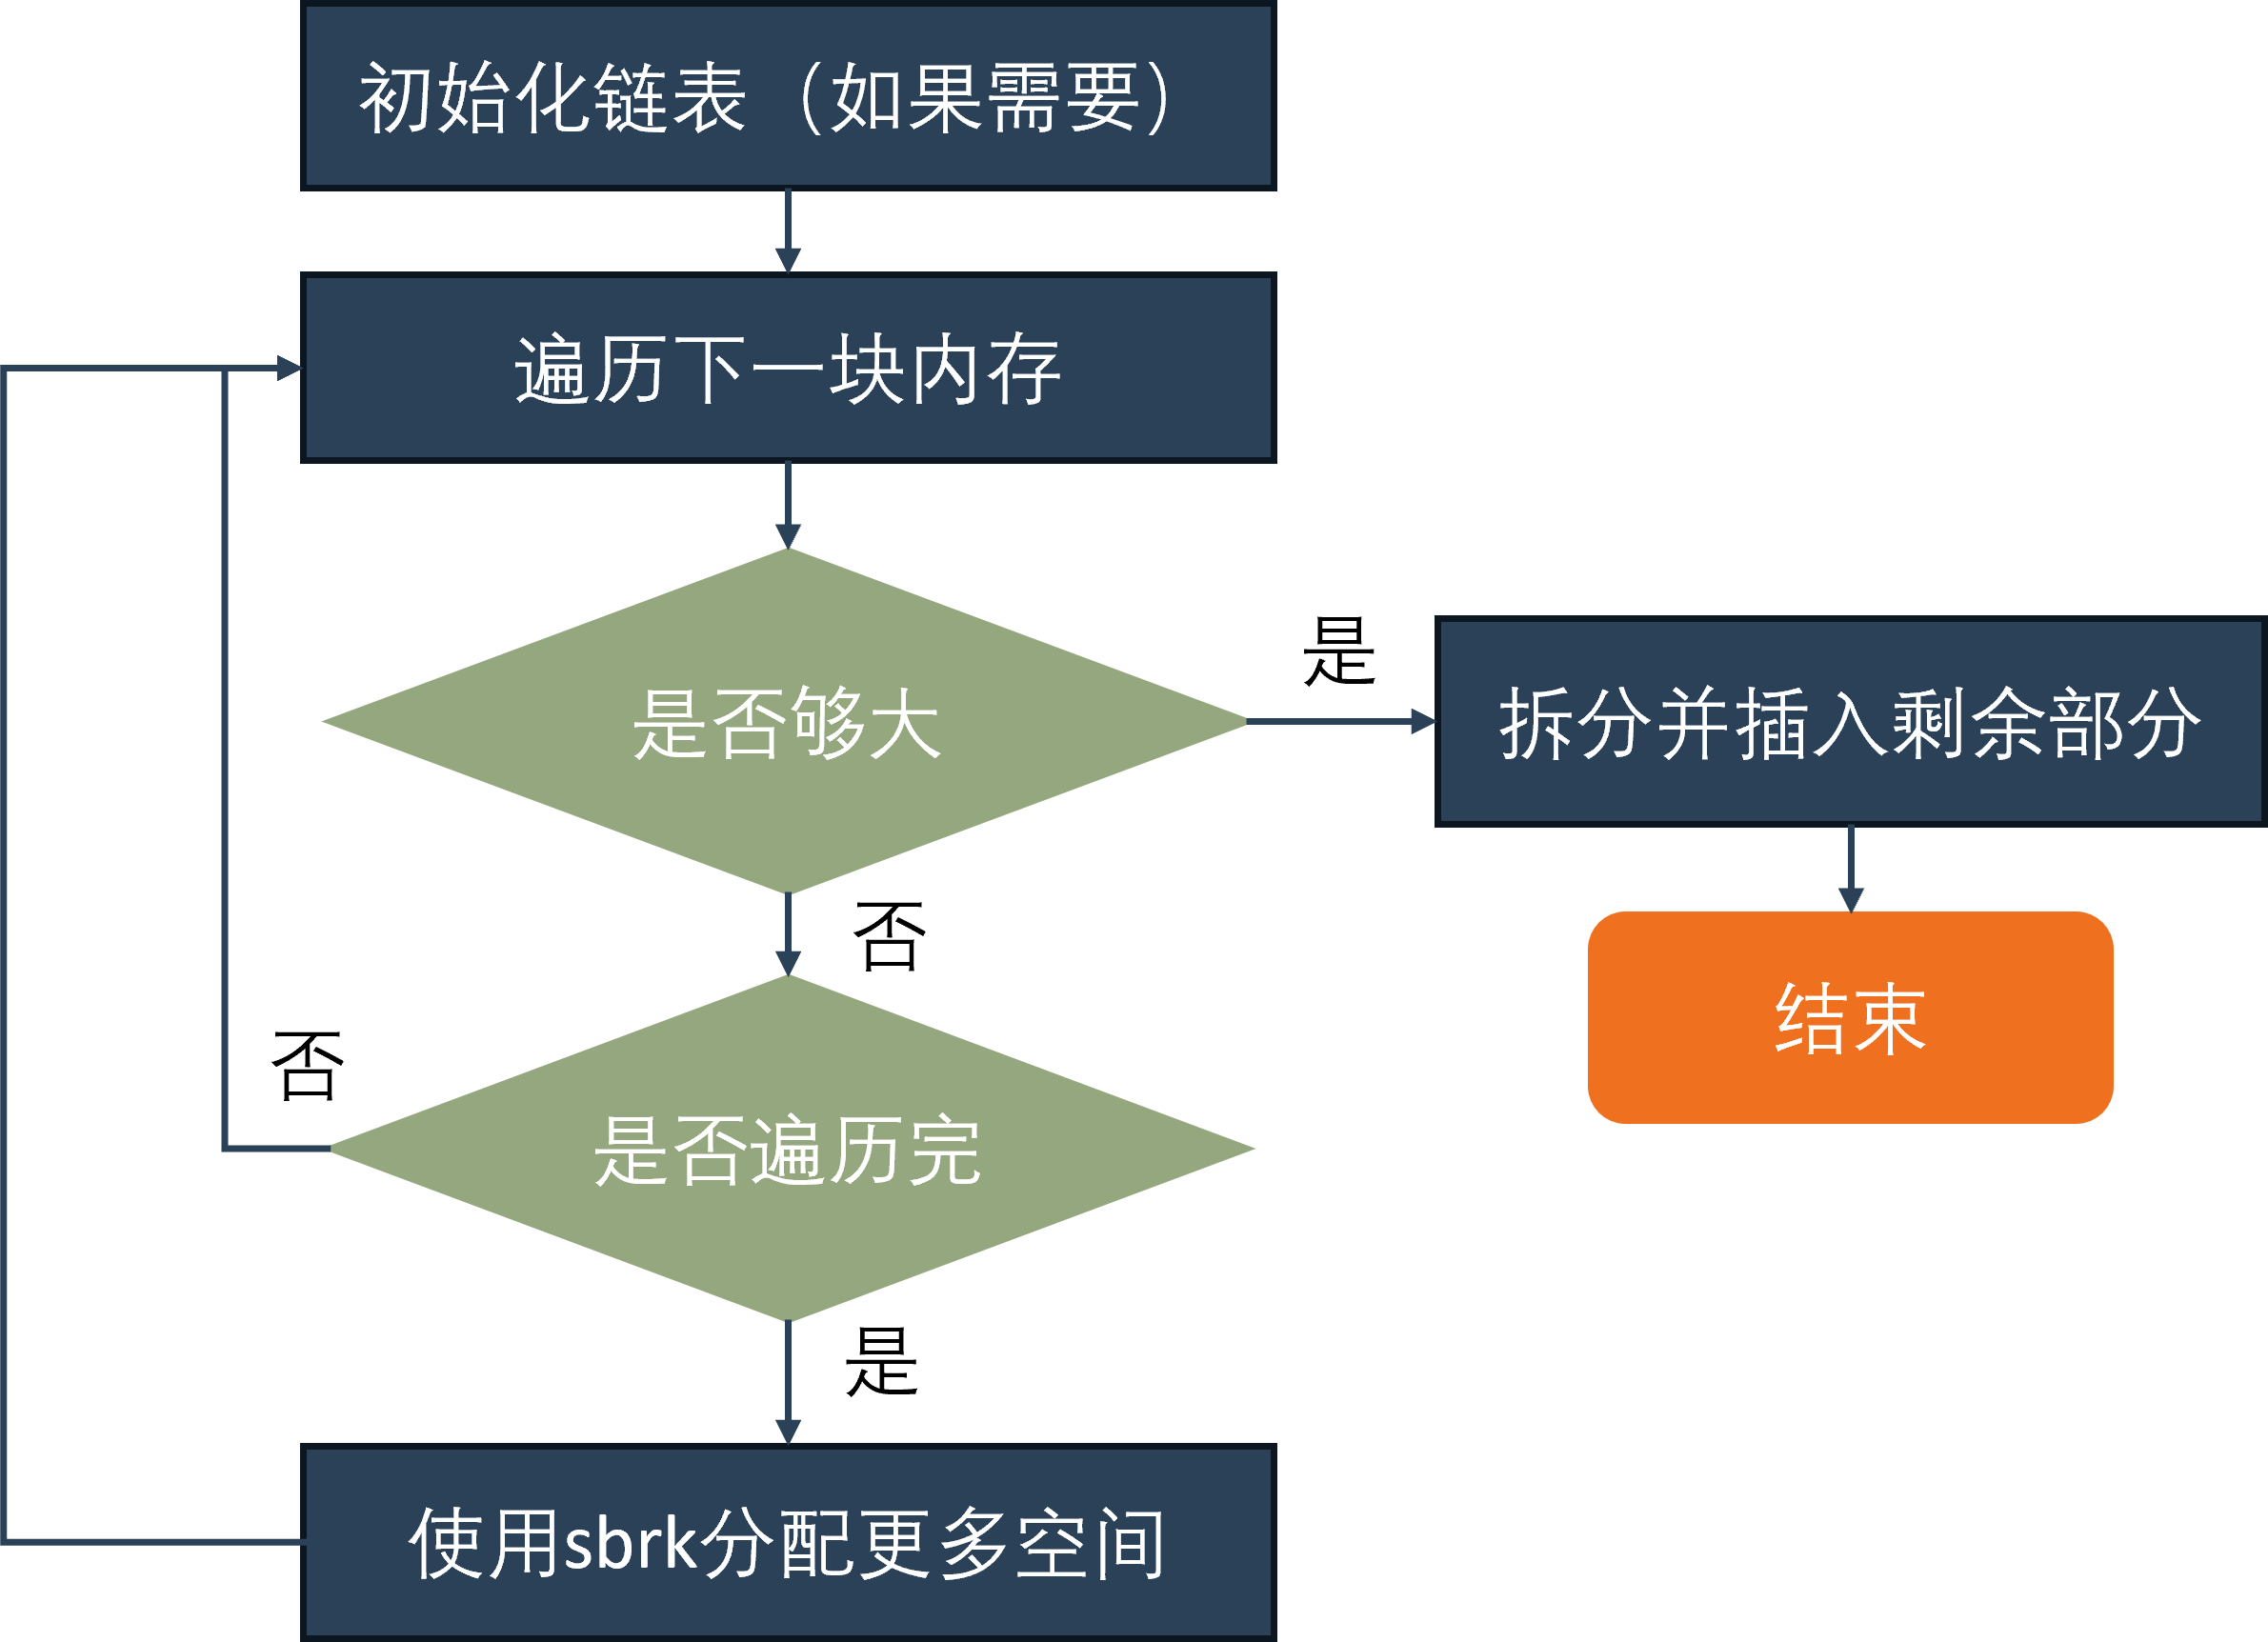
\includegraphics[width=0.4\textwidth]{images/ff.png}
\end{figure}


\subsection{\texttt{free}}

该函数会遍历链表,找到内存地址合适的位置,将块插入。此外,还会合并相邻的空闲块。

\subsection{\texttt{calloc}}

\texttt{calloc}分配指定大小的内存并置为0,这是通过调用\texttt{ff\_malloc}并使用\texttt{memset}赋值实现的。

\subsection{\texttt{test.c}}

该程序使用并测试了首次适配的分配和释放功能,它进行三轮测试,
每轮测试都是连续分配逐渐增大大小的内存块并写入数据,并输出相应信息。
最后,对这些内存块进行释放。

\section{实现最佳适应算法}

最佳适配算法中\texttt{free}、\texttt{calloc}的实现都与首次适配相同,
只需要修改具体的分配逻辑。在分配时遍历整个链表,选择与所要求尺寸差值最小的
块进行分配,如代码~\ref{code:findclose}。
\begin{listing}[htb]
	\caption{查找最接近的内存块}
	\label{code:findclose}
	\inputminted[firstline=84,lastline=106]{c}{../code/3/bf_malloc.c}
\end{listing}
当找到这样的块时,采用和首次适配相同的拆分策略,并返回相应的内存。
如果没有找到这样的块,则使用\texttt{sbrk}系统调用分配内存,
将新的块插入链表中,然后再次调用\texttt{bf\_malloc}进行分配。
由于这次一定能找到合适的块,因此不会再次调用\texttt{bf\_malloc}。
因此,这种做法不会带来过多的额外开销。如代码~\ref{code:sbrk}。
\begin{listing}[htb]
	\caption{处理找不到块的情况}
	\label{code:sbrk}
	\inputminted[firstline=136,lastline=159]{c}{../code/3/bf_malloc.c}
\end{listing}

\subsection{对比}

为了对比两种不同的分配算法,我进一步修改代码,在每次分配成功以后输出整个空闲链表的内容,其中0代表头节点,如图~\ref{fig:cmpffbf}。
\begin{figure}[htb]
	\centering
	\caption{使用不同的策略分配内存}
	\label{fig:cmpffbf}
	\begin{subfigure}{0.45\textwidth}
		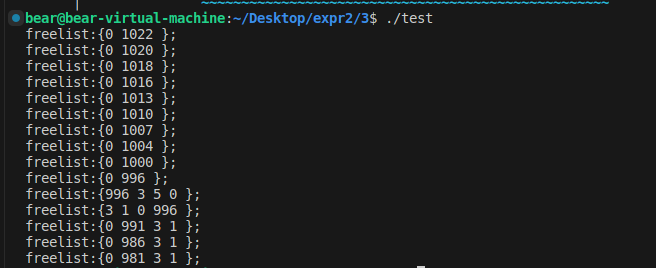
\includegraphics[width=0.9\textwidth]{images/ff_fl.png}
	\end{subfigure}
	\begin{subfigure}{0.45\textwidth}
		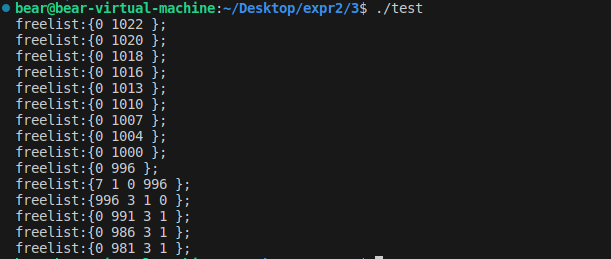
\includegraphics[width=0.9\textwidth]{images/bf_fl.png}
	\end{subfigure}
\end{figure}
首先,测试函数会进行10次内存分配,然后释放一部分块,此时根据输出,有三个空闲的内存块,
它们的长度分别是7,5,996。

此后的分配中,首次适配和最佳适配将表现出差别:接下来,会分配大小为4的块。
此时,首次适配找到块7,拆分后返回。这是,剩下的三块为3,5,996。而最佳适配策略
会找出与请求尺寸大小最接近的块,则会找到块5,进行拆分后剩余的内存块为7,1,996。

一方面,最佳适配会遍历整个链表,查找的时间会更长。假设有$n$个块,每个块成为最佳适配的概率则为$\frac{1}{n}$。
那么最佳适配的查找长度的数学期望为:
\begin{equation}
	\label{eqn:bf}
 	\mathbb{E}[L] = \sum_{i=1}^{n} \frac{i}{n} = \frac{n+1}{2}
\end{equation}
而首次适配中,每个块平均情况下能否被选中的次数大致相等,则选中的概率为$\frac{1}{2}$,
选择第一块的概率为$\frac{1}{2}$,选择第二块的概率为$\frac{1}{2}\times \left(1-\frac{1}{2}\right)$,以此类推。
查找长度的期望为:
\begin{equation}
	\label{eqn:ff}
 	\mathbb{E}[L] = \sum_{i=1}^{n} \frac{1}{2^n}\times n = \left(2-\frac{1}{2^{n-1}}\right)-\frac{n}{2^n}
\end{equation}
显然,比较\eqref{eqn:bf}和\eqref{eqn:ff},当$n$足够大时,首次适配的查找长度更短。

另一方面,首次适配可能拆分较大的内存块,导致剩余的内存块较小,而最佳适配则会尽量保留较大的内存块。
然而,由图~\ref{fig:cmpffbf}中的例子可以看出,最佳适配的效果并不好,因为它留下大量可能无法再分配的细碎的内存块,例如上例中的大小为1的块。
这会导致内存碎片的显著增加。


\section{实验总结}

本次实验让我更深入地了解了Linux内存分配和管理的原理和方法,以及各种算法的实现。通过实践,我学会了如何使用\texttt{kmalloc()}和\texttt{vmalloc()}函数,
并学会了如何实现first fit算法和best fit算法。在实践过程中进一步锻炼了内核模块编程和算法实现的能力。
在进行实验的过程中,我还学会了如何查找Linux系统内核的文档,并且更了解了Linux操作系统的运作方式和内部结构,这对于我今后的学习和研究都有很大的帮助。


\end{spacing}

\end{document}